\documentclass{article}
\usepackage[utf8]{inputenc}

\usepackage{float}
\usepackage{caption}

\RequirePackage{tabularx}

\usepackage[table]{xcolor} 
\definecolor{myblue}{HTML}{CCF4FF}
\definecolor{myorange}{HTML}{FCAD68}

\usepackage{tikz}
\tikzstyle{decision} = [diamond, draw, fill=myblue, 
text width=4.5em, text badly centered, node distance=2.5cm, inner sep=0pt]
\tikzstyle{block} = [rectangle, draw, 
fill=myblue, align=center, rounded corners, minimum width = 2cm, minimum height=1cm]
\tikzstyle{line} = [draw, -latex']

\begin{document}
\pagestyle{empty}
\large

\section*{\hspace{-1cm}3D printers - Handleiding}

TODO: maak deze handleiding. 

doel van de handleidng : na het lezen moet een SA de workflow van het 3D printen kunnen snappen
\begin{figure}[H]
\centering
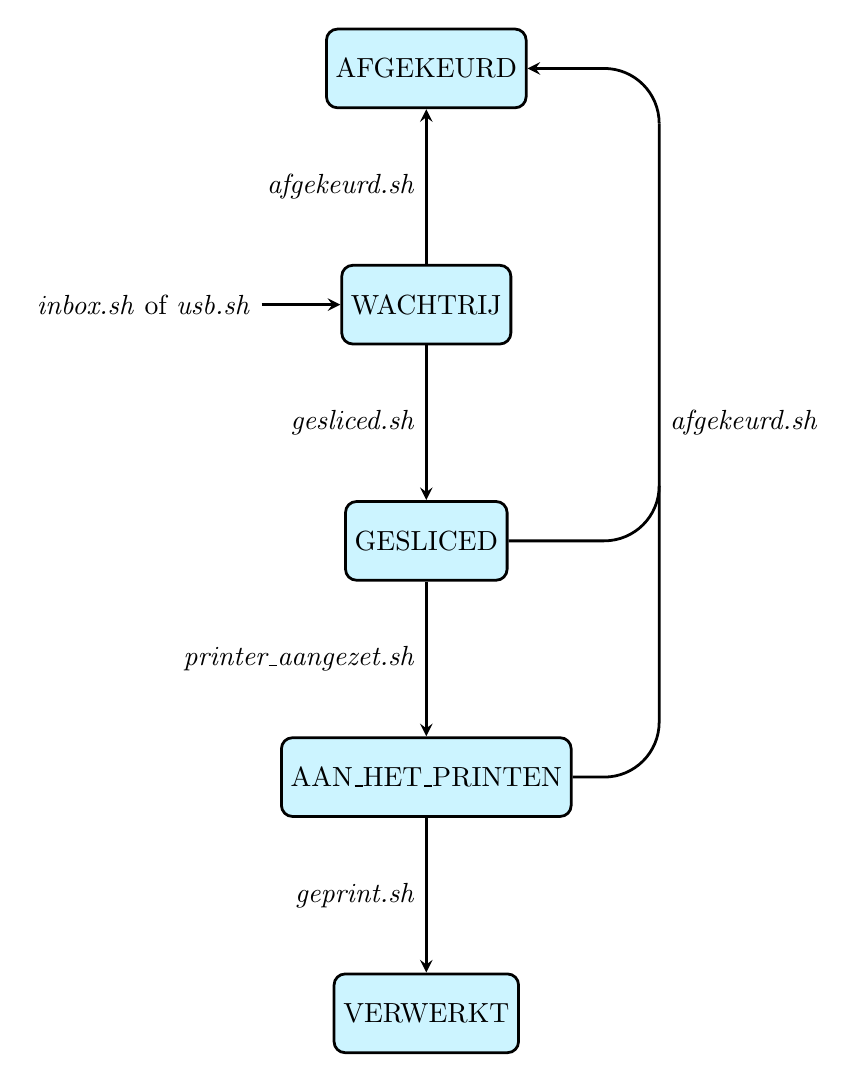
\begin{tikzpicture}[node distance = 3.0cm, line width=1pt]
    % Nodes
    \node [block] (wachtrij) {WACHTRIJ};
    \node [block, above of=wachtrij]  (afgekeurd) {AFGEKEURD};
    \node [block, below of=wachtrij]  (gesliced) {GESLICED};
    \node [block, below of=gesliced]  (aan_het_printen) {AAN\_HET\_PRINTEN};
    \node [block, below of=aan_het_printen] (verwerkt) {VERWERKT};

    % define lengths
 \pgfmathsetlengthmacro{\alpha}{0.7cm} % curve radius
  \pgfmathsetlengthmacro{\negalpha}{-\alpha}
  \pgfmathsetlengthmacro{\beta}{0.4cm} % straight bit before the curve


    % arrows
  \draw[>=stealth, ->, line width=1.0pt] ([xshift=-1.0cm]wachtrij.west) to node[xshift=-0.5cm,left]{\textit{inbox.sh} of \textit{usb.sh}} (wachtrij.west);
\draw[>=stealth, ->, line width=1.0pt] (wachtrij.north) to node[left] {\textit{afgekeurd.sh}} (afgekeurd.south);
\draw[>=stealth, ->, line width=1.0pt] (wachtrij.south) to node[left] {\textit{gesliced.sh}} (gesliced.north);

\draw[>=stealth, -, line width=1.0pt] (aan_het_printen.east) -- ++(\beta,0)  to[out=0, in=-90] ++(\alpha, \alpha) -- node[right]{\textit{afgekeurd.sh}} ([xshift=\alpha+\beta,yshift=\negalpha]afgekeurd.east -| aan_het_printen.east);
    \draw[>=stealth, <-, line width=1.0pt] (afgekeurd.east) -- ([xshift=\beta] afgekeurd -| aan_het_printen.east)  to[out=0, in=90] ++(\alpha,\negalpha);


    \draw[>=stealth, -, line width=1.0pt] (gesliced.east) -- ([xshift=\beta] gesliced -| aan_het_printen.east) to[out=0, in=-90] ++(\alpha,\alpha);

  \draw[>=stealth, ->, line width=1.0pt] (gesliced.south) to node[left] {\textit{printer\_aangezet.sh}} (aan_het_printen.north);
      \draw[>=stealth, ->, line width=1.0pt] (aan_het_printen.south) to node[left] {\textit{geprint.sh}} (verwerkt.north);

\end{tikzpicture}
\caption*{\textbf{Workflow gaat zo}, ingeleverde .stl bestanden worden door \textit{bash} functies verplaatst van/naar de folders aangegeven met hoofdletters.}%
\end{figure}

\section*{\hspace{-1cm}Functie Beschrijving:}
\begin{table}[H]
    \centering
    \rowcolors{2}{gray!25}{white}
    \begin{tabular}%
    {>{\raggedright\arraybackslash}p{0.20\textwidth}%
    |>{\raggedright\arraybackslash}p{0.80\textwidth}}
    \rowcolor{myblue}
    Functie & beschrijving\\\hline
  \textit{inbox.sh}& Vraag of alle \textit{x} binnengekomen mails of een enkele ($x=1$) mail behandeld moet worden. Bij een enkele mail selecteer welke via interactief keuzemenu in de terminal.\newline Maak voor iedere mail die .stl bestanden bevat een folder aan in met naam /Documents/WACHTRIJ/\textit{naam}/ waarbij \textit{naam} de naam is van de persoon die de mail heeft gestuurd. Download de .stl attachments en de binnen gekomen mail naar de respectivelijke \textit{naam} folder. Maak voor ieder van de \textit{x} folders een \textit{afkeur.sh}functie en plaats deze in de respectivelijke \textit{naam} folder.\\

\textit{usb.sh}& Vraag of alle \textit{x} binnengekomen mails of een enkele ($x=1$) mail behandeld moet worden. Bij een enkele mail selecteer welke via interactief keuzemenu in de terminal.\newline Maak voor iedere mail die .stl bestanden bevat een folder aan in met naam /Documents/WACHTRIJ/\textit{naam}/ waarbij \textit{naam} de naam is van de persoon die de mail heeft gestuurd. Download de .stl attachments en de binnen gekomen mail naar de respectivelijke \textit{naam} folder. Maak voor ieder van de \textit{x} folders een \textit{afkeur.sh}functie en plaats deze in de respectivelijke \textit{naam} folder.\\



\textit{afgekeurd.sh}& Verplaats de inhoud van de folder waarin \textit{afgekeurd.sh}zich bevind van de WACHTRIJ of GESLICED\_PRINTEN folder naar de Documents/AFGEKEURD/\textit{MM}-\textit{DD}\_\textit{naam} folder, hierbij is \textit{MM-DD} vandaag. Popup een mail reactie voor met de 'afkeur' handtekening voor de SA om aan te passen en te versturen.\\
\textit{gesliced.sh}& Vraag of alle \textit{y} folders in WACHTRIJ of een enkele ($y=1$) folder behandeld moet worden. Bij een enkele folder selecteer welke via interactief keuzemenu in de terminal. Plaats de inhoud van de \textit{y} folders van WACHTRIJ/\textit{naam} in \textit{y} GESLICED\_PRINTEN/\textit{hh}h\_\textit{mm}m\_\textit{naam}/ folders, hierbij is \textit{hh} het aantal uren van de print en \textit{mm} het aantal minuten van de print.
Maak voor ieder van de \textit{y} folders een \textit{geprint.sh}functie en plaats deze in de respectivelijke \textit{hh}h\_\textit{mm}m\_\textit{naam} folder.
    \\
\textit{geprint.sh}& Verplaats de inhoud van GESLICED\_PRINTEN/\textit{hh}h\_\textit{mm}m\_\textit{naam}/ naar VERWERKT/\textit{MM}-\textit{DD}\_\textit{hh}h\_\textit{mm}m\_\textit{naam}/ waarbij \textit{MM-DD} vandaag is. Popup een mail reactie met de 'geprint' handtekening voor een SA om aan te passen en te versturen.\\
    \end{tabular}
    \caption*{}%
\end{table}


\end{document}

